\documentclass[10pt,a4paper]{article}
\usepackage{amsmath}
\usepackage{amssymb}
\usepackage{graphicx}
\usepackage{color}
\usepackage{fancyhdr}
\usepackage{fancyvrb}
\usepackage[margin=3.5cm]{geometry}
\usepackage{framed}
\usepackage{enumerate}
\usepackage{textcomp}
\def\ket#1{\left|#1\right\rangle}
\def\bra#1{\left\langle#1\right|}
\def\braket#1{\left\langle#1\right\rangle}

\FrameSep 8pt
\setlength{\topsep}{1pt}

\definecolor{linkcol}{rgb}{0.0, 0.0, 0.5}
\usepackage[colorlinks=true,urlcolor=linkcol,citecolor=black,linkcolor=linkcol]{hyperref}

\renewcommand\thesection{7.\arabic{section}}
\renewcommand\thesubsection{\thesection.\arabic{subsection}}

\fancyhf{}
\lhead{\tiny Y.~D.~Chong (2016)}
\rhead{\scriptsize MH2801: Complex Methods for the Sciences}
\lfoot{}
\rfoot{\thepage}
\pagestyle{fancy}

\makeatletter
\def\PY@reset{\let\PY@it=\relax \let\PY@bf=\relax%
    \let\PY@ul=\relax \let\PY@tc=\relax%
    \let\PY@bc=\relax \let\PY@ff=\relax}
\def\PY@tok#1{\csname PY@tok@#1\endcsname}
\def\PY@toks#1+{\ifx\relax#1\empty\else%
    \PY@tok{#1}\expandafter\PY@toks\fi}
\def\PY@do#1{\PY@bc{\PY@tc{\PY@ul
\def\PYZdl{\char`\$}
\def\PYZhy{\char`\-}
\def\PYZsq{\char`\'}
\def\PYZdq{\char`\"}
\def\PYZti{\char`\~}

\begin{document}
\setcounter{page}{46}
\noindent
\underline{\textbf{\LARGE 7. Branch Points and Branch Cuts}}
\vskip 0.1in
    
When introducing complex algebra, we postponed discussion of what it
means to raise a complex number to a non-integer power, such as
$z^{1/2}$, $z^{4/3}$, or $z^{\pi}$. It is now time to open that
particular can of worms. This involves learning about the two
indispensible concepts of \textbf{branch points} and \textbf{branch
  cuts}.

\section{Non-integer powers as multi-valued operations}
\label{non-integer-powers-as-multi-valued-operations}

Given a complex number in its polar representation, $z =
r\exp[i\theta]$, raising to the power of $p$ could be handled this
way:
\begin{equation}
  z^p = \left(re^{i\theta}\right)^p = r^p e^{ip\theta}.
\end{equation}
In this expression, let's take a closer look at the complex
exponential term $e^{ip\theta}$. Since $\theta = \mathrm{arg}(z)$ is
an angle, we can change it by any integer multiple of $2\pi$ without
altering the value of $z$. Taking this fact into account, we can
re-write the above equation as
\begin{align}
  z^p &= \left(r\,e^{i(\theta + 2\pi n)}\right)^p \\
  &= \left(r^p e^{ip\theta} \right) e^{2\pi i n p} \quad\;
  \mathrm{where}\;\; n\in\mathbb{Z}.
\end{align}
In other words, the fact that the argument is an angle gives rise to
an extra factor of $\exp(2\pi i n p)$. If $p$ is an integer, then
$2\pi n p$ is an integer multiple of $2\pi$, in which case $z^p$ has
the same value regardless of $n \in \mathbb{Z}$:
\begin{align}
  z^p &= \left(r\,e^{i(\theta + 2\pi n)}\right)^p \\
  &= r^p e^{ip\theta} \;\;\mathrm{for\;all}\;\; n\in\mathbb{Z}
  \;\;\;(\text{if}\,p\in\mathbb{Z}).
\end{align}
On the other hand, if $p$ is not an integer, then there is no unique
answer, since $\exp\left(2 \pi i np\right)$ can have multiple possible
values depending on the choice of $n \in \mathbb{Z}$. In such cases,
``raising to the power of $p$'' is a \textbf{multi-valued operation}.
This means it cannot be treated as a function in the usual sense,
since the basic definition of a function states that it must have
unambiguous outputs.

\subsection{Roots of unity}
\label{roots-of-unity}

Let's take a closer look at the problematic exponential term,
\begin{equation}
  \exp\left(2\pi i np\right), \quad n \in \mathbb{Z}.
\end{equation}
If $p$ is irrational, $2\pi np$ never repeats itself modulo $2\pi$. So
we have an infinite number of different results for $z^p$, one for
each integer $n$, where each result is equally legitimate!

More interesting is the case of a non-integer \emph{rational} power,
which can be written as $p = P/Q$, where $P$ and $Q$ are integers with
no common divisor. Then it can be shown that $2\pi n\, (P/Q)$ has $Q$
unique values modulo $2\pi$:
\begin{equation}
  2\pi n\, \left(\frac{P}{Q}\right)
  = 2\pi \times \left\{0,\, \frac{1}{Q},\, \frac{2}{Q},\, \dots, \frac{(Q-1)}{Q} \right\} \quad(\mathrm{modulo} \; 2\pi).
\end{equation}
Note that this set is independent of the numerator $P$; it turns out
that $P$ only affects the sequence in which these numbers are
generated. We can clarify this using a few simple examples.

\begin{framed}
\label{square-root-example}
\noindent
\underline{\textbf{Example}}
\vskip 0.02in \noindent
Consider the complex square root operation, $z^{1/2}$. We can write
$z$ as
\begin{equation}
z = r e^{i\theta}.
\end{equation}
Then,
\begin{equation}
z^{1/2} = \left[r \, e^{i(\theta + 2 \pi n)} \right]^{1/2} = r^{1/2} \, e^{i\theta/2} \, e^{i \pi n}, \quad n \in \mathbb{Z}.
\end{equation}
The factor of $e^{i\pi n}$ takes on two possible values: $+1$ for
even $n$, and $-1$ for odd $n$. Hence,
\begin{equation}
z^{1/2} = \Big\{ \;\; r^{1/2} \, e^{i\theta/2} \;\; \mathrm{or} \;\;
-r^{1/2} \, e^{i\theta/2} \Big\}.
\end{equation}
We can write this more compactly as:
\begin{equation}
z^{1/2} = r^{1/2} \, e^{i\theta/2} \;\times\; \left\{1, -1\right\}.
\end{equation}
\end{framed}

\begin{framed}
\noindent
\underline{\textbf{Example}}
\vskip 0.02in \noindent
Consider the cube root operation $z^{1/3}$. Again, we write $z$ in
its polar representation:
\begin{equation}
z^{1/3} = r^{1/3} \, e^{i\theta/3} \, e^{2\pi i n/3}, \quad n \in \mathbb{Z}.
\end{equation}
The multi-valuedness comes $\exp(2\pi i n/3)$, which takes the
following values:
\begin{equation*}
\begin{array}{|c||c|c|c|c|c|c|c|c|c|} \hline n &\cdots & -2 & -1 & 0 & 1 & 2 & 3 & 4 & \cdots \\ \hline e^{2\pi i n/3} &\cdots & e^{2\pi i /3} & e^{-2\pi i /3} & \;\,\;1\;\,\; & e^{2\pi i /3} & e^{-2\pi i /3} & \;\,\;1\;\,\; & e^{2\pi i /3} & \cdots \\ \hline \end{array}
\end{equation*}
From the pattern, we can figure out that
\begin{equation}
  e^{2\pi i n/3} = \left\{1, e^{2\pi i /3}, e^{-2\pi i /3}\right\}.
\end{equation}
Therefore, the cube root operation has three distinct values:
\begin{equation}
  z^{1/3} = r^{1/3} \, e^{i\theta/3} \;\times\;
  \left\{1, e^{2\pi i /3}, e^{-2\pi i /3}\right\}.
\end{equation}
\end{framed}

\begin{framed}
\noindent
\underline{\textbf{Example}}
\vskip 0.02in \noindent
Consider the operation $z^{2/3}$. Again, we write $z$ in its polar
representation, and obtain
\begin{equation}
z^{2/3} = r^{2/3} \, e^{2i\theta/3} \, e^{4\pi i n/3}, \quad n \in \mathbb{Z}.
\end{equation}
The multi-valuedness comes from $\exp(4\pi i n/3)$.  For different
$n$, the values are:
\begin{equation*}
\begin{array}{|c||c|c|c|c|c|c|c|c|c|} \hline n &\cdots & -2 & -1 & 0 & 1 & 2 & 3 & 4 & \cdots \\ \hline e^{4\pi i n/3} &\cdots & e^{-2\pi i /3} & e^{2\pi i /3} & \;\,\;1\;\,\; & e^{-2\pi i /3} & e^{2\pi i /3} & \;\,\;1\;\,\; & e^{-2\pi i /3} & \cdots \\ \hline \end{array}
\end{equation*}
Hence, there are three possible values of this exponential factor,
\begin{equation}
  e^{2\pi i n (2/3)} = \left\{1, e^{2\pi i /3}, e^{-2\pi i /3}\right\}.
\end{equation}
This is the same set of values obtained for $e^{2\pi i n/3}$, but in a
different order.  Thus,
\begin{equation}
  z^{2/3} = r^{2/3} \, e^{2i\theta/3} \;\times\;
  \left\{1, e^{2\pi i /3}, e^{-2\pi i /3}\right\}.
\end{equation}
\end{framed}

From these examples, we can deduce the following general expression
for a complex rational-power operation:
\begin{equation}
  z^{P/Q} = r^{P/Q} \; e^{i\theta\, (P/Q)}\, \times
  \left\{1,\, e^{2\pi i \cdot (1/Q)},\, e^{2\pi i \cdot (2/Q)},\, \dots, e^{2\pi i \cdot [(1-Q)/Q]} \right\}.
\end{equation}
The quantities in the curly brackets are called the \textbf{$Q$-roots
  of unity}. In the complex plane, they sit at $Q$ evenly-spaced
positions along the unit circle, with $1$ (unity) as one of the
values, as shown in the following figure:

\begin{figure}[h]
  \centering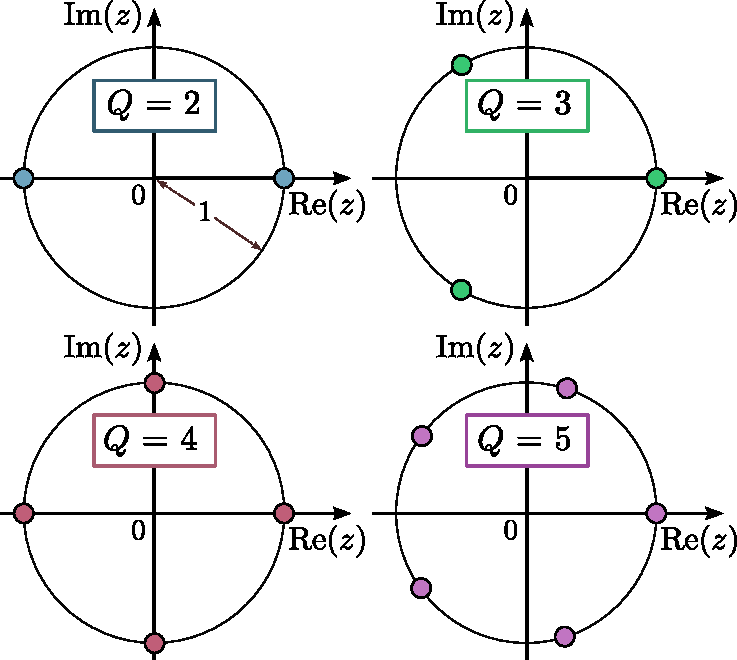
\includegraphics[width=0.53\textwidth]{roots_of_unity}
\end{figure}
    
\subsection{Complex logarithms}
\label{complex-logarithms}

Here is another way to think about the problem of non-integer powers.
Recall what it means to raise a number to, say, the power of 5: we
simply multiply the number by itself five times. What about raising a
number to a non-integer power $p$? For the real case, we used the
following definition based on a combination of exponential and
logarithm functions:
\begin{equation}
  x^p \equiv \exp\,\left[\,p\ln(x)\right].
\end{equation}
This definition relies on the fact that, for real inputs, the
logarithm is a well-defined function. That, in turn, comes from the
definition of the logarithm as the inverse of the exponential
function. Since the real exponential is a one-to-one function, it has
a well-defined inverse which is also a one-to-one function.

For complex numbers, however, the exponential function is many-to-one,
not one-to-one. Specifically, changing its input by any multiple of
$2\pi i$ gives the same value:
\begin{equation}
  \exp(z + 2\pi i n) = \exp(z) \cdot e^{2\pi i n}
  = \exp(z) \quad \forall\; n \in \mathbb{Z}.
\end{equation}
The inverse of the complex exponential is the \textbf{complex
  logarithm}. Since the complex exponential is many-to-one, the
complex logarithm does not produce a single unique output for each
input $z$.  Instead, $\ln(z)$ refers to an infinite discrete set of
values, separated by integer multiples of $2\pi i$. We can express
this state of affairs in the following way:
\begin{equation}
  \ln(z) = \big[\ln(z)\big]_{\mathrm{p.v.}}\;
  +\; 2 \pi i n, \quad n \in \mathbb{Z}.
\end{equation}
Here, $[\ln(z)]_{\mathrm{p.v.}}$ denotes the \textbf{principal value}
of $\ln(z)$, which refers to a ``standardized'' value of the logarithm
operation (which we'll define later). Do not think of the principal
value as the ``actual'' result of the $\ln(z)$ operation! There are
multiple possible results, each equally legitimate; we simply decide
to pick one of them as a ``reference'' result for convenience.

We now return to our definition of the ``raising a number to the power
of $p$'' operation, which is the aforementioned formula $z^p \equiv
\exp\left[p\ln(z)\right]$. If we let $\ln(z)$ in this formula be the
complex logarithm, then the multi-valuedness of the complex logarithm
gives
\begin{align}
  z^p &= \exp\Big\{p\big([\ln(z)]_{\mathrm{p.v.}} + 2\pi i n\big)\Big\}\\
  &= \exp\Big\{p[\ln(z)]_{\mathrm{p.v.}}\Big\} \times e^{2\pi i np},
  \quad n \in \mathbb{Z}.
\end{align}
The final factor, which is responsible for the multi-valuedness, are
the roots of unity discussed in the \hyperref[roots-of-unity]{previous
  section}.

\section{Branches}\label{branches}

We have discussed two examples of multi-valued complex operations:
taking non-integer powers, and the complex logarithm. Most of the
multi-valued operations typically encountered in practice are variants
of these. However, we usually prefer to deal with functions rather
than multi-valued operations. One major motivating factor is that the
concept of the complex derivative was formulated in terms of
functions, not multi-valued operations.

There is a standard procedure to convert multi-valued operations into
functions. Firstly, we define one or more curve(s) in the complex
plane, called \textbf{branch cuts} (the reason for this name will be
explained later). Next, we retrict the domain (the set of permissible
inputs) to exclude all values of $z$ lying on a branch cut. For this
restricted domain, the outputs of the multi-valued operation can be
grouped into discrete \textbf{branches}, with each branch behaving
just like a function.

The above procedure is best understood by working through the
following example.

\subsection{Branches of the complex square root}
\label{branches-of-the-complex-square-root}

The complex square root, $z^{1/2}$, is a multi-valued operation.  We
\hyperref[square-root-example]{saw in Section \ref{roots-of-unity}}
that it gives two possible values, i.e.~there are two branches. To
define the branches of the complex square root, we can perform the
following steps:

\begin{enumerate}
\item
Define a branch cut along the negative real axis. We restrict the
domain by excluding values of $z$ along the branch cut; in other
words, we will only deal with complex numbers whose polar
representation can be written as
\begin{equation}
z = r e^{i\theta}, \quad \theta \in (-\pi, \pi).
\end{equation}
(For those unfamiliar with this mathematical notation,
$\theta \in (-\pi, \pi)$ refers to the interval
$-\pi < \theta < \pi$. The parentheses in $(-\pi, \pi)$ indicates
that the boundary values of $-\pi$ and $\pi$ are excluded. By
contrast, we would write $\theta \in [-\pi, \pi]$ to refer to the
interval $-\pi \le \theta \le \pi$, with the square brackets
indicating that the boundary values are to be included.)

\item
Observe that the square root has two possible values, corresponding to
the \hyperref[roots-of-unity]{2-roots of unity}. If we consistently
pick the $+1$ root, that defines one branch of the square root. In
this branch, for any $z = re^{i\theta}$ away from the branch cut, the
value of the square root is
\begin{equation}
  f_+(z) = r^{1/2} \, e^{i\theta/2}, \quad \theta \in (-\pi, \pi).
\end{equation}
This branch can be regarded as a well-defined function with
unambiguous outputs.

\item
Picking the $-1$ root gives us another branch, corresponding to the
function
\begin{equation}
f_-(z) = -r^{1/2} \, e^{i\theta/2}, \quad \theta \in (-\pi, \pi).
\end{equation}
This branch can also be regarded as a well-defined function with
unambiguous outputs.
\end{enumerate}

\noindent
In the following plot, you can observe how varying $z$ affects the
positions of $f_+(z)$ and $f_-(z)$ in the complex plane:

\begin{figure}[h]
  \centering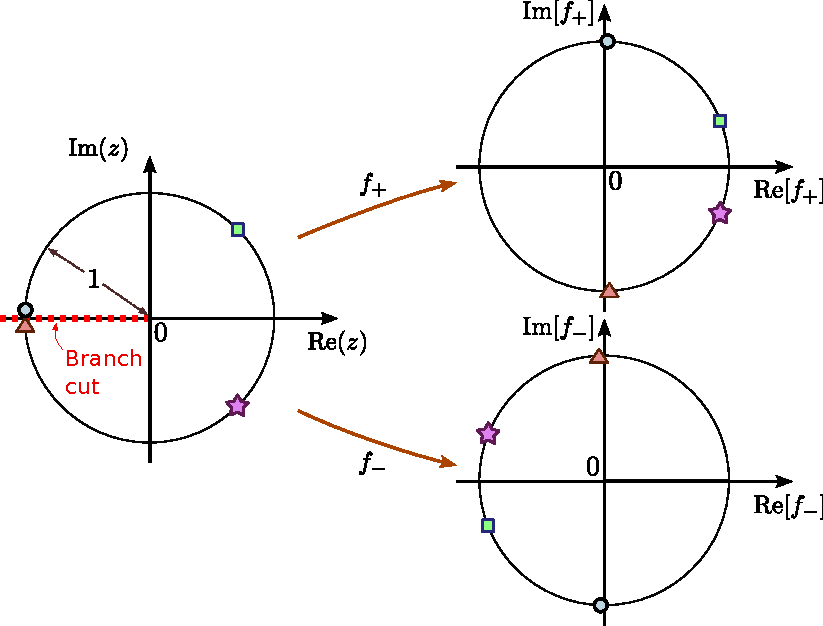
\includegraphics[width=0.77\textwidth]{complex_root_1}
\end{figure}

The left-hand figure shows the complex plane for $z$.  The red dashes
indicate the branch cut, which lies on the negative real axis.  This
is because we represent the argument of $z$ as $\theta \in
(-\pi,\pi)$, excluding $\theta = \pm \pi$.  Consistent with this
choice of branch cut, the complex square root has two branch
functions, $f_+(z)$ and $f_-(z)$.  The different symbols on the
left-hand figure indicate four particular values of $z$ in the complex
plane; the same symbols on the right-hand figures show the
corresponding values of $f_+(z)$ and $f_-(z)$.

Observe that the values of $f_+(z)$ all lie in the right half of the
complex plane, i.e., having arguments $\in (-\pi/2, \pi/2)$.  The
values of $f_-(z)$ all lie in the left half of the complex plane.

Each of the branch functions, $f_+(z)$ and $f_-(z)$, are not merely
well-defined functions; they are in fact analytic functions over all
of the complex plane except the branch cut. This fact can be proven
using the Cauchy-Riemann equations, which is left as an exercise.

The end-point of the branch cut is called a \textbf{branch point},
which occurs at $z = 0$.  At this point, both branches give the same
result: $f_+(0) = f_-(0) = 0$. We will have more to say about branch
points \hyperref[branch-points]{shortly}.

\subsection{Different branch cuts for the complex square root}

You may be wondering why the branch cut lies along the negative real
axis. In fact, this choice is not unique.

For instance, we could place the branch cut along the positive real
axis. This corresponds to specifying the input $z$ using a different
interval for $\theta$:
\begin{equation}
  z = re^{i\theta}, \quad \theta \in (0, 2\pi).
\end{equation}
Next, we use the same formulas as before to define the branches of the
complex square root:
\begin{equation}
  f_\pm(z) = \pm r^{1/2} \, e^{i\theta/2}.
\end{equation}
But because the domain of $\theta$ has been changed to $(0, 2\pi)$,
the set of inputs $z$ now excludes the positive real axis. With this
new choice of branch cut, the branches are shown in the following
figure:

\begin{figure}[h]
  \centering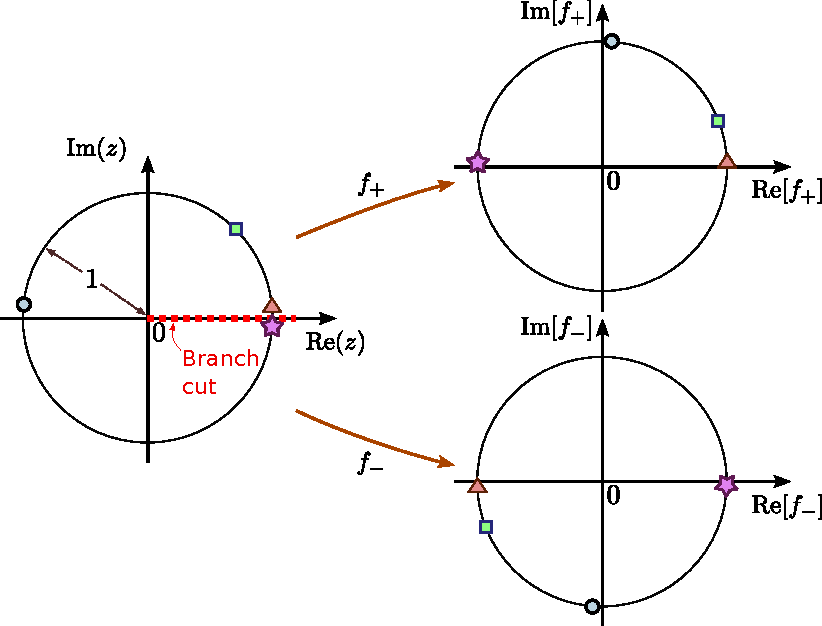
\includegraphics[width=0.75\textwidth]{complex_root_2}
\end{figure}

The two branch functions are different from what we had before. Now,
the value of $f_+(z)$ always lies in the upper half of the complex
plane, while $f_-(z)$ is always in the lower half of the complex
plane. However, the value of both branches remains the same at the
branch point: $f_+(0) = f_-(0) = 0$.

The branch cut serves as a kind of boundary where the two branches are
``glued'' together. You can think of ``crossing'' a branch cut as
having the effect of moving continuously from one branch to
another. In the above figure, consider the value of $z$ corresponding
to the red triangle, which lies just above the branch cut. Observe
that the corresponding value of $f_+(z)$ lies just above the positive
real axis, while $f_-(z)$ lies just below the negative real
axis.

Next, consider the value of $z$ corresponding to the purple star,
which lies just below the branch cut.  Moving from the triangle to the
star is equivalent to a small downwards displacement of $z$,
``crossing'' the branch cut.  Observe that the new value of $f_-(z)$
lies just below the positive real axis, close to where $f_+(z)$ was
previously. Conversely, $f_+(z)$ now lies just above the negative real
axis, close to where $f_-(z)$ was previously.  In other words,
crossing the branch cut had the effect of moving values from one
branch to another.

\subsection{Branch points}
\label{branch-points}

The tip of each branch cut is called a \textbf{branch point}. More
precisely, a branch point is a point $z$ where the multi-valued
operation gives an unambiguous answer, with different branches giving
the same output. Whereas the choice of branch cuts is non-unique, the
positions of the branch points of a multi-valued operation are
uniquely determined. The branch points for the two most
commonly-encountered multi-valued operations are simple to remember:
\begin{itemize}
\item
  The $z^p$ operation (for non-integer $p$) has branch points at
  $z = 0$ and $z = \infty$. For rational powers $p = P/Q$, where
  $P$ and $Q$ have no common divisor, there are $Q$ distinct
  branches, one for each root of unity. At each branch point, all $Q$
  branches meet.
\item
  The \hyperref[complex-logarithms]{complex logarithm} has branch
  points at $z = 0$ and $z = \infty$. There is an infinite series of
  branches, separated from each other by multiples of $2 \pi i$. At
  each branch point, all of these branches meet.
\end{itemize}

We can readily understand why both $z^p$ and $\ln(z)$ have branch
points at $z = 0$ and $z = \infty$. First, notice that at $z = 0$, the
only possible value of $z^p$ is $0$, regardless of the choice of the
root of unity. Hence, $z^p$ must have a branch point at $z = 0$.  But
due to the \hyperref[complex-logarithms]{relation between rational
  powers and the complex logarithm}, $z^p \equiv \exp[p\ln(z)]$, this
implies that $\ln(z)$ likewise has a branch point at $z = 0$. (The
fact that $\ln(z)$ is singular at $z = 0$ doesn't prevent this from
being a branch point.) Then, because of the property
\begin{equation}
\ln\left(\frac{1}{z}\right) = -\ln(z),
\end{equation}
the branch point at $z = 0$ implies that $\ln(z)$ also has a branch
point at $z = \infty$. This, in turn, implies that $z^p$ has a
branch point at $z = \infty$.

\section{Branch cuts for general multi-valued operations}
\label{branch-cuts-for-general-multi-valued-operations}

Having discussed the simplest multi-valued operations, $z^p$ and
$\ln(z)$, here is how to assign branch cuts for more general
multi-valued operations. This is a two-step process:

\begin{enumerate}
\item
Locate the \hyperref[branch-points]{branch points}. In most of the
examples that we will encounter, the multi-valuedness arises
ultimately from the \hyperref[complex-logarithms]{complex logarithm},
and in such cases the branch points are the values of $z$ such that
the input to the logarithm is $0$ or $\infty$.

\item
Assign \hyperref[branches]{branch cuts} in the complex plane, such
that:
\begin{itemize}
\item Every branch point has a branch cut ending on it.
\item Every branch cut ends on a branch point.
\end{itemize}
Note that any branch point lying at infinity must also obey these rules.
The branch cuts should not intersect.
\end{enumerate}

\noindent
It is worth emphasizing again that branch points are independent of
the choice of branch cuts. Each branch point is, by definition, a
point where the multi-valued operation becomes single-valued. For the
operations $z^p$ and $\ln(z)$, the branch points are at $z=0$ and $z =
\infty$, but for other operations they may occur at other positions in
the complex plane.

The choice of where to place branch cuts is not unique. Branch cuts are
usually chosen to be straight lines, for simplicity, but this is not
necessary. The various choices of branch cuts simply correspond to
different ways of partitioning the multi-valued operation's various
values into distinct branches.

\subsection{An important example}
\label{an-important-example}

Here is an important non-trivial example of a multi-valued operation
made up of complex logarithms:
\begin{equation}
f(z) = \ln(z+1) - \ln(z-1).
\end{equation}
This is multi-valued because of the presence of the complex logarithm.
The branch points occur where the inputs to the logarithms are either
zero or infinite. The former occurs when $z = 1$ and $z = -1$.

It might seem also that $z = \infty$ could also be a branch point, but
this is not the case.  That's because we can write
\begin{equation}
f(z) = \ln\left(\frac{z+1}{z-1}\right).
\end{equation}
The input to the logarithm goes to 1 for $z = \infty$. In a sense, the
branch points at infinity from the two logarithms ``cancel each other
out''. So there are only two branch points, at $z = 1$ and $z = -1$.
We can assign any branch cut that joins these two. A convenient choice
is shown below:

\begin{center}
  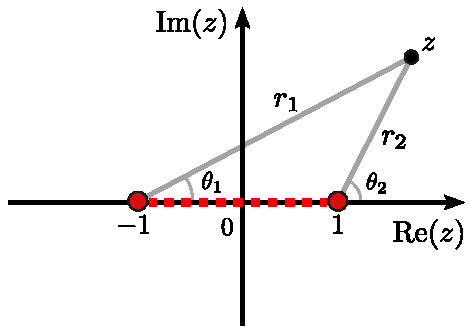
\includegraphics[width=0.4\textwidth]{branch_cut_example}
\end{center}

This choice of branch cut is nice because we can express the $z+1$ and
$z - 1$ terms using the polar representations
\begin{equation}
  z + 1 = r_1\,e^{i\theta_1}, \quad z - 1 = r_2\, e^{i\theta_2},
\end{equation}
where $r_1$, $r_2$, $\theta_1$, and $\theta_2$ are shown
graphically in the above figure. The positioning of the branch cut
corresponds to a particular choice for the ranges of the complex
arguments $\theta_1$ and $\theta_2$. As we'll shortly see, the
present choice of branch cut corresponds to
\begin{equation}
  \theta_1 \in (-\pi,\pi), \quad \theta_2 \in (-\pi,\pi).
\end{equation}
In terms of this polar representation, $f(z)$ can be written as
\begin{equation}
  f(z) = \ln\left(\frac{r_1}{r_2}\right) + i(\theta_1 - \theta_2 + 2\pi m), \quad m\in\mathbb{Z}
\end{equation}
where
\begin{equation*}
  z = -1 + r_1\,e^{i\theta_1} = 1 + r_2\,e^{i\theta_2},\quad\theta_1, \theta_2 \in (-\pi,\pi).
\end{equation*}
The choice of integer $m$ specifies the branch, and $m = 0$ is
conventionally assumed to be the principal branch.

Let's now verify that setting $\theta_1 \in (-\pi,\pi)$ and
$\theta_2 \in (-\pi,\pi)$ is consistent with our choice of branch cut.
Consider the principal branch, and compare the outputs of the above
formula for $z$ just above the real axis, and for $z$ just below the
real axis. There are three cases of interest. Firstly, for
$\mathrm{Re}(z) < 1$ (to the left of the leftmost branch point),
\begin{align}
  \mathrm{Im}(z) &= 0^+ \;\;\Rightarrow\;\;
  f(z) = \ln\left(\frac{r_1}{r_2}\right) + i\Big((\pi) - (\pi)\Big) \quad
  = \ln\left(\frac{r_1}{r_2}\right) \\
  \mathrm{Im}(z) &= 0^- \;\;\Rightarrow \;\;
  f(z) = \ln\left(\frac{r_1}{r_2}\right) + i\Big((-\pi) - (-\pi)\Big)
  = \ln\left(\frac{r_1}{r_2}\right).
\end{align}
Thus, there is no discontinuity along this segment of the real axis.

Secondly, for $-1 < \mathrm{Re}(z) < 1$ (between the two branch
points),
\begin{align}
  \mathrm{Im}(z) &= 0^+ \;\;\Rightarrow\;\; f(z)
  = \ln\left(\frac{r_1}{r_2}\right) + i\Big((0) - (\pi)\Big) \;\;
  = \ln\left(\frac{r_1}{r_2}\right) -i\pi \\
  \mathrm{Im}(z) &= 0^- \;\;\Rightarrow\;\;
  f(z) = \ln\left(\frac{r_1}{r_2}\right) + i\Big((0) - (-\pi)\Big)
  = \ln\left(\frac{r_1}{r_2}\right) + i\pi.
\end{align}
Hence, in the segment between the two branch points, there is a
discontinuity of $\pm 2\pi i$ on different sides of the real axis. The
value of this discontinuity is exactly equal, of course, to the
separation between the different branches of the complex logarithm.

Finally, for $\mathrm{Re}(z) > 1$ (to the right of the rightmost
branch point), there is again no discontinuity:
\begin{align}
  \mathrm{Im}(z) &= 0^+ \;\;\Rightarrow\;\; f(z)
  = \ln\left(\frac{r_1}{r_2}\right) + i\Big((0) - (0)\Big)
  = \ln\left(\frac{r_1}{r_2}\right) \\
  \mathrm{Im}(z) &= 0^- \;\;\Rightarrow\;\;
  f(z) = \ln\left(\frac{r_1}{r_2}\right) + i\Big((0) - (0)\Big)
  = \ln\left(\frac{r_1}{r_2}\right).
\end{align}

\section{Exercises}\label{exercises}

\begin{enumerate}
\item
Find the values of $(i)^i$.

\item
For each of the following multi-valued functions, find all the possible
function values, at the specified $z$:

\begin{enumerate}
\item $z^{1/3}$ at $z = 1$.
\item $z^{3/5}$ at $z = i$.
\item $\ln(z+i)$ at $z = 1$.
\item $\cos^{-1}(z)$ at $z = i$
\end{enumerate}

\item
For the square root operation $z^{1/2}$, choose a branch cut. Then
show that both the branch functions $f_\pm(z)$ are analytic over all
of $\mathbb{C}$ excluding the branch cut.

\item
Consider $f(z) = \ln(z+a) - \ln(z-a)$. For simplicity, let $a$ be a
positive real number. As \hyperref[an-important-example]{discussed in
  Section \ref{an-important-example}}, we can write this as
\begin{equation}
  f(z) = \ln\left|\frac{z+a}{z-a}\right|
  + i(\theta_+ - \theta_-), \qquad \theta_\pm \equiv \mathrm{arg}(z\pm a).
\end{equation}
Suppose we represent the arguments as $\theta_+ \in (-\pi,\pi)$ and
$\theta_- \in (-\pi,\pi)$. Explain why this implies a branch cut
consisting of a straight line joining $a$ with $-a$. Using this
representation, calculate the change in $f(z)$ over an infinitesimal
loop encircling $z = a$ or $z = -a$. Calculate also the change in
$f(z)$ over a loop of radius $R \gg a$ encircling the origin (and thus
enclosing both branch points).
\end{enumerate}
    
\end{document}
